%\documentclass[12pt]{article}

\questionheader{ex:s1.7}


%%%%%%%%%%%%%%%%%%
\subsection*{\Conceptual}
%%%%%%%%%%%%%%%%%%

%%%%%%%%%%%%%%%%%%%%%%%%%%%%%%%%
\begin{question}[M200 2008A] %7
Match the following equations and expressions with the corresponding 
pictures. Cartesian coordinates are $(x, y, z)$, cylindrical coordinates 
are $(r, \theta, z)$, and spherical coordinates are $(\rho, \theta, \varphi)$.

\begin{center}
 (A) \raisebox{-0.5\height}
           {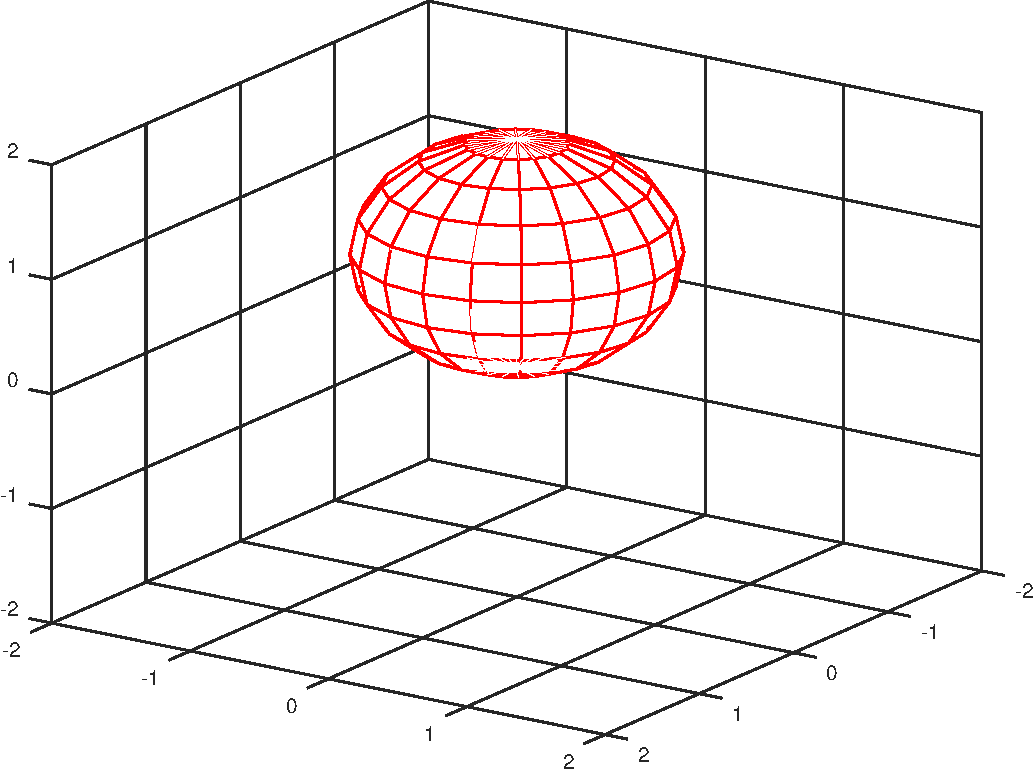
\includegraphics[width=0.33\textwidth, height=0.3\textwidth]
                                                   {fig/surface1.pdf}}
\qquad
  (B) \raisebox{-0.5\height}
            {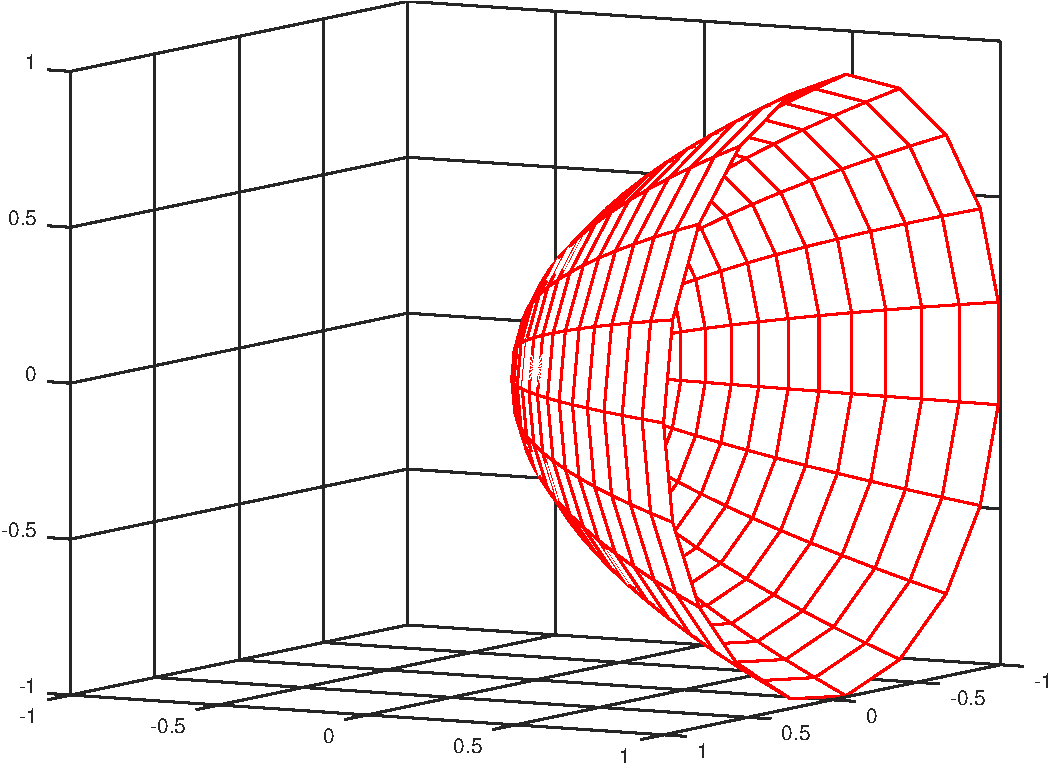
\includegraphics[width=0.33\textwidth, height=0.33\textwidth]
                                                   {fig/surface2.pdf}}
\end{center}
\begin{center}
  (C) \raisebox{-0.5\height}
            {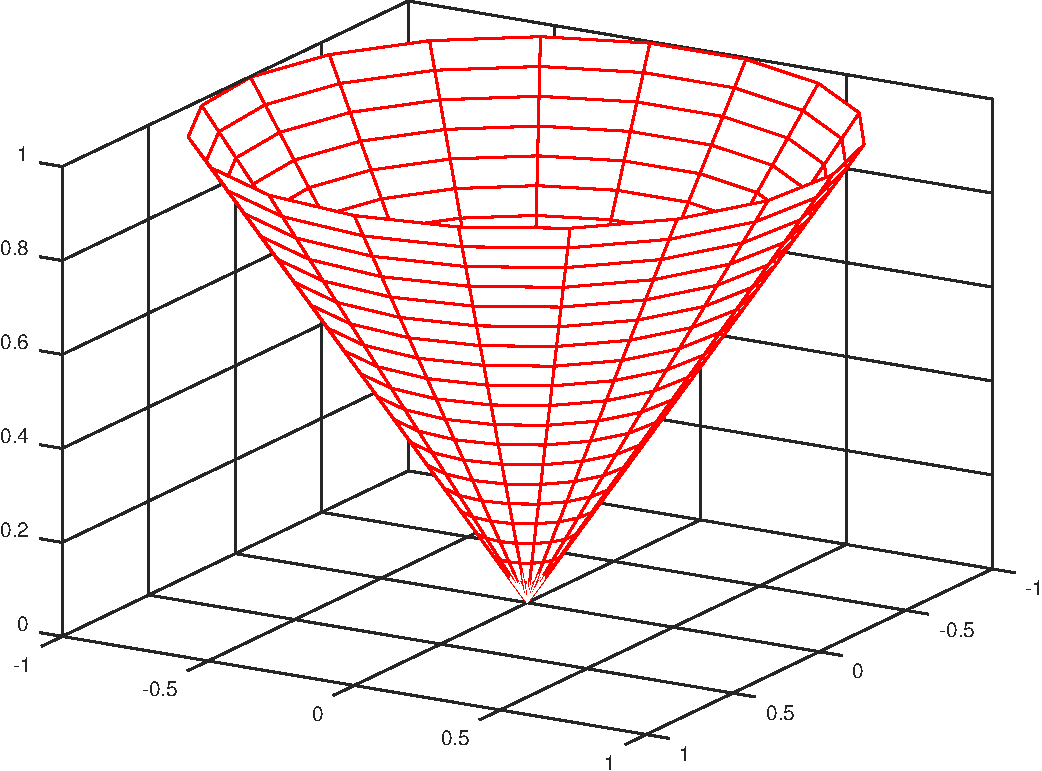
\includegraphics[width=0.33\textwidth, height=0.33\textwidth]
                                                   {fig/surface3.pdf}}
\qquad
  (D)  \raisebox{-0.5\height} 
            { 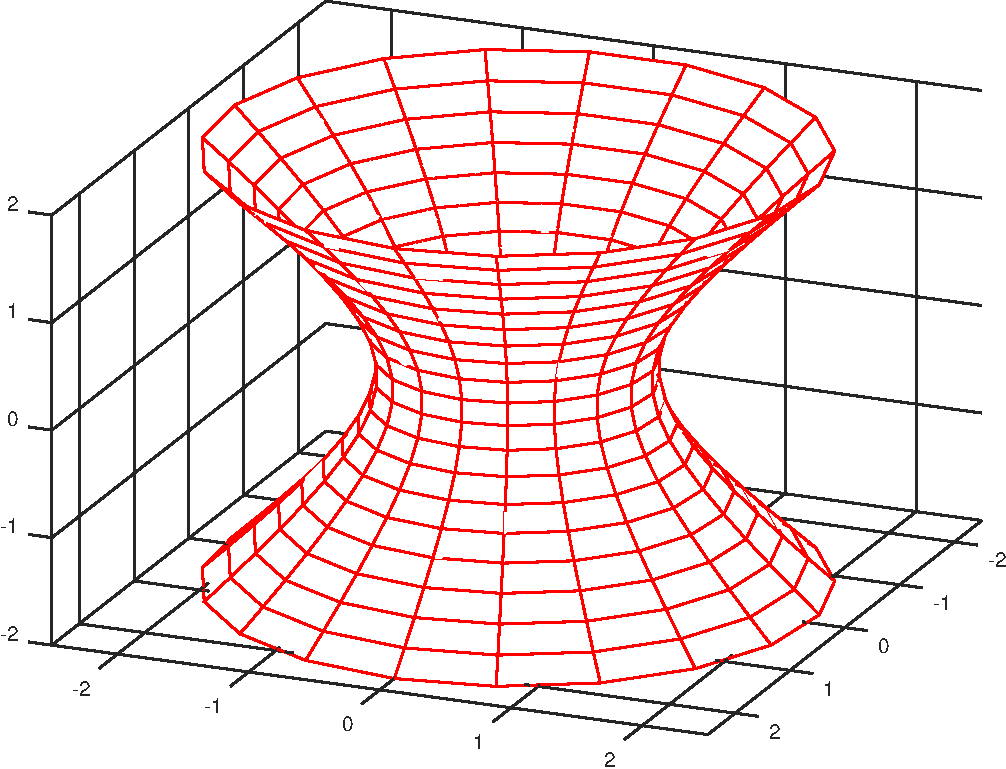
\includegraphics[width=0.33\textwidth, height=0.3\textwidth]
                                                    {fig/surface4.pdf}}
\end{center}
\begin{center}
 (E) \raisebox{-0.5\height}
           { 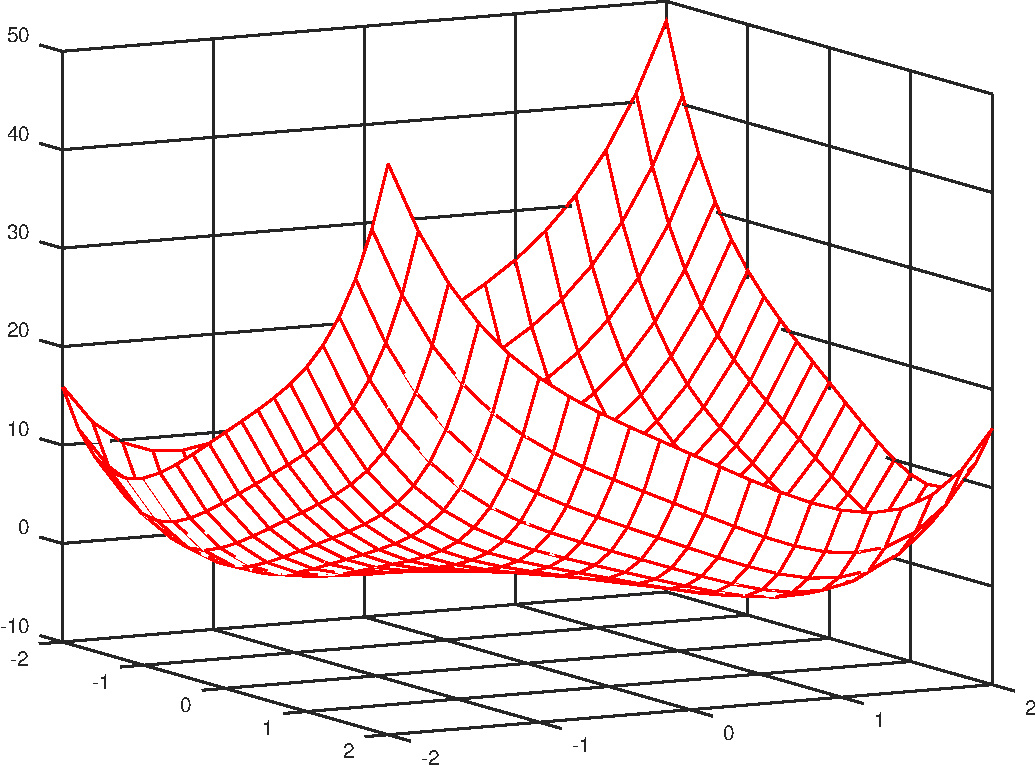
\includegraphics[width=0.33\textwidth, height=0.3\textwidth]
                                                    {fig/surface5.pdf}}
\qquad
  (F) \raisebox{-0.5\height}
           {  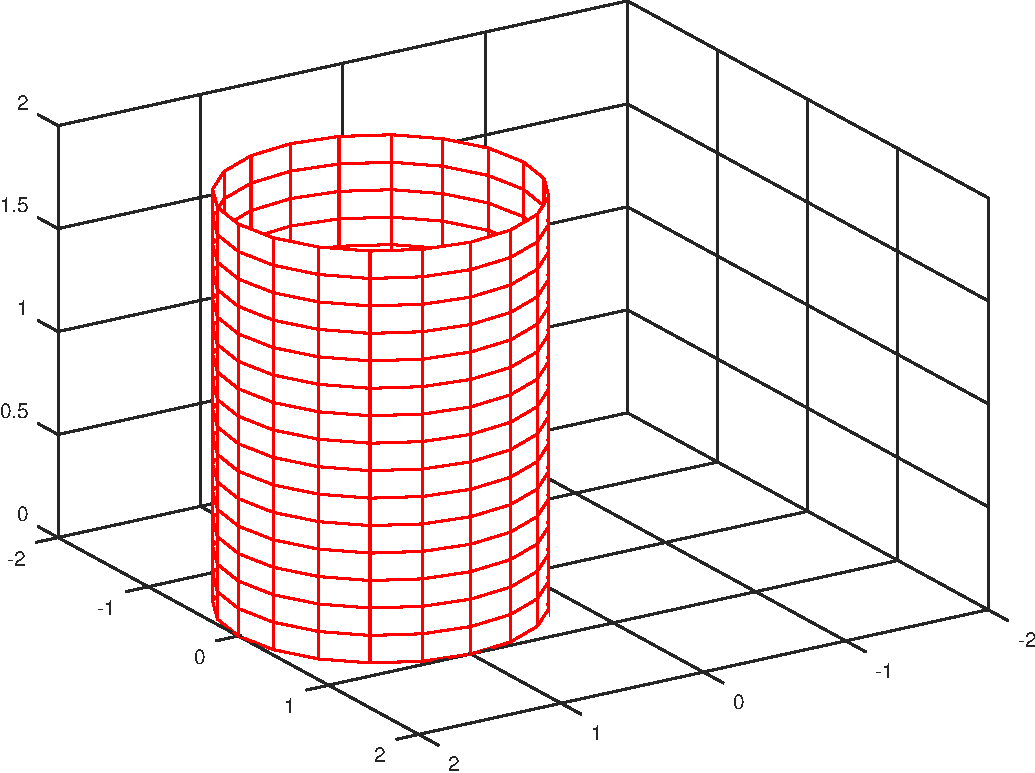
\includegraphics[width=0.33\textwidth, height=0.3\textwidth]
                                                    {fig/surface6a.pdf}}
\end{center}

\begin{alignat*}{7}
&\text{(a)}\quad& \varphi&=\pi/3 &
&\text{(b)}\quad& r&=2\cos\theta &
&\text{(c)}\quad& x^2+y^2&=z^2+1 \\
&\text{(d)}& y&=x^2+z^2\qquad &
&\text{(e)}& \rho&=2\cos\varphi\qquad &
&\text{(f)}& z&=x^4+y^4-4xy &
\end{alignat*}
\end{question}

%\begin{hint}
%
%\end{hint}

\begin{answer}
(a) $\leftrightarrow$ (C) \qquad
(b) $\leftrightarrow$ (F) \qquad
(c) $\leftrightarrow$ (D) \qquad
(d) $\leftrightarrow$ (B) \qquad
(e) $\leftrightarrow$ (A) \qquad
(f) $\leftrightarrow$ (E)
\end{answer}

\begin{solution}
(a) $\varphi =\frac{\pi}{3}$ is a surface of constant (spherical coordinate)
$\varphi$. So it is a cone with vertex at the origin. We can express
$\varphi=\frac{\pi}{3}$ in cartesian coordinates by observing that
$0\le\varphi\le\frac{\pi}{2}$ so that $z\ge 0$, and
\begin{align*}
\varphi=\frac{\pi}{3}
\iff
\tan\varphi =\frac{\sqrt{3}}{2}
\iff
\rho\sin\varphi =\frac{\sqrt{3}}{2}\rho\cos\varphi
\iff
\sqrt{x^2+y^2}=\frac{\sqrt{3}}{2} z
\end{align*}
So the picture that corresponds to (a) is (C).

(b) As $r$ and $\theta$ are cylindrical coordinates
\begin{align*}
r=2\cos\theta
\iff
r^2=2 r\cos\theta
\iff
x^2+y^2 = 2x
\iff
(x-1)^2+y^2=1
\end{align*}
There is no $z$ appearing in $(x-1)^2+y^2=1$. So every constant $z$
cross--section of $(x-1)^2+y^2=1$ is a (horizontal) circle of radius
$1$ centred on the line $x=1$, $y=0$. It is a cylinder of radius $1$
centred on the line $x=1$, $y=0$.
So the picture that corresponds to (b) is (F).

(c) Each constant $z$ cross--section of $x^2+y^2=z^2+1$ is a (horizontal)
circle centred on the $z$--axis. The radius of the circle is $1$
when $z=0$ and grows as $z$ moves away from $z=0$.  So
$x^2+y^2=z^2+1$ consists of a bunch of (horizontal) circles stacked
on top of each other, with the radius increasing with $|z|$. It
is a hyperboloid of one sheet. 
The picture that corresponds to (c) is (D).

(d) Every point of $y=x^2+z^2$ has $y\ge 0$. Only (B) has that 
property. We can also observe that every constant $y$ cross--section
is a circle centred on $x=z=0$. The radius of the circle is zero
when $y=0$ and increases as $y$ increases. The surface $y=x^2+z^2$
is a paraboloid.
The picture that corresponds to (d) is (B).

(e) As $\rho$ and $\varphi$ are spherical coordinates
\begin{align*}
\rho=2\cos\varphi
\iff
\rho^2=2\rho\cos\varphi
\iff
x^2+y^2+z^2=2z
\iff
x^2+y^2 + (z-1)^2=1
\end{align*}
This is the sphere of radius $1$ centred on $(0,0,1)$.
The picture that corresponds to (e) is (A).

(f) The only possibility left is that the picture that
corresponds to (f) is (E).
\end{solution}

%%%%%%%%%%%%%%%%%%%%%%%%%%%%%%%%
\begin{question}
In each of (a) and (b) below, you are provided with a sketch of the first quadrant parts of a few level curves of some function $f(x,y)$.
Sketch the first octant part of the corresponding graph $z=f(x,y)$.
\begin{center}
 (a) \raisebox{-0.5\height}
           {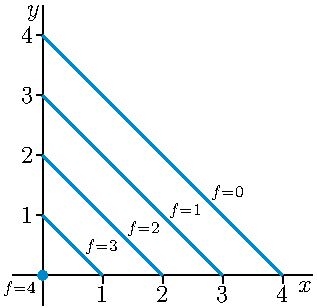
\includegraphics[width=0.33\textwidth, height=0.3\textwidth]
                                                   {fig/planeLevelA.pdf}}
\qquad
  (b)\ \ \raisebox{-0.5\height}
            {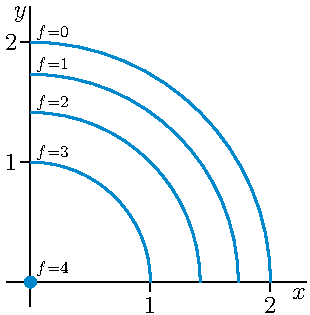
\includegraphics[width=0.33\textwidth, height=0.33\textwidth]
                                                   {fig/paraboloidLevelA.pdf}}
\end{center}
\end{question}

\begin{hint}
For each $C$, redraw the level curve $f(x,y)=C$ in the plane $z=C$.
\end{hint}


\begin{answer}
\begin{center}
 (a) \raisebox{-0.5\height}
           {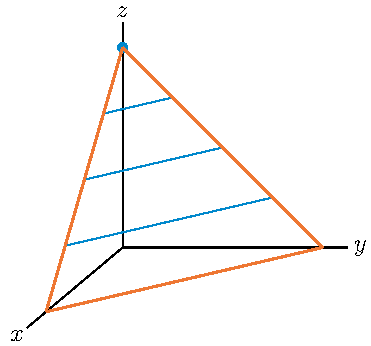
\includegraphics[width=0.4\textwidth, height=0.4\textwidth]
                                                   {fig/planeGraphB.pdf}}
\qquad
  (b)\ \ \raisebox{-0.45\height}
            {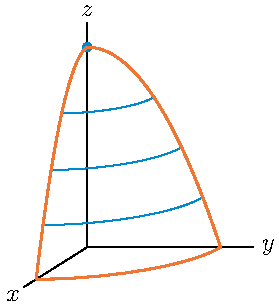
\includegraphics[width=0.33\textwidth, height=0.33\textwidth]
                                                   {fig/paraboloidGraphB.pdf}}
\end{center}
\end{answer}


\begin{solution}
Each solution below consists of three sketchs.
\begin{itemize}
\item 
In the first sketch, we just redraw the given level curves with the
$x$- and $y$-axes reoriented so that the sketch looks like we are high on the $z$-axis looking down at the $xy$-plane.

\item 
In the second sketch, we lift up each level curve $f(x,y)=C$ and draw it in 
the horizontal plane $z=C$. That is we draw 
\begin{align*}
&\Set{(x,y,z)}{f(x,y)=C,\ z=C,\ x\ge 0, y\ge 0} \\
&\hskip1in=\Set{(x,y,z)}{z=f(x,y),\ z=C,\ x\ge 0, y\ge 0}
\end{align*}

\item
Finally, in the third sketch, we draw the part of graph $z=f(x,y)$ in the
first octant, just by ``filling in the gaps in the second sketch''.
\end{itemize}

(a)
\begin{center}
  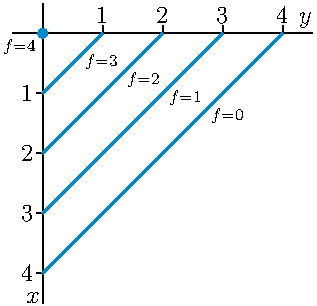
\includegraphics{fig/planeLevelB.pdf}
\qquad
  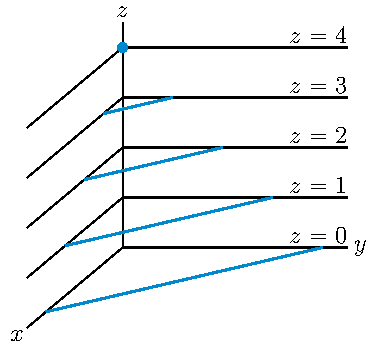
\includegraphics{fig/planeGraphA.pdf}
\end{center}

\begin{center}
  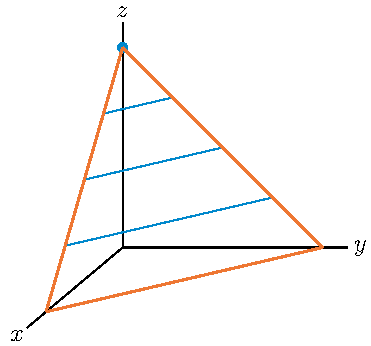
\includegraphics{fig/planeGraphB.pdf}
\end{center}


(b)
\begin{center}
  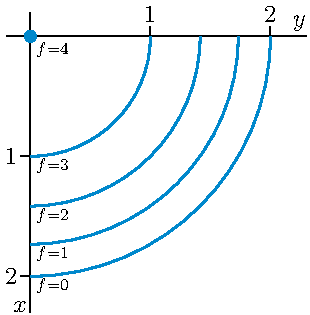
\includegraphics{fig/paraboloidLevelB.pdf}
\qquad
  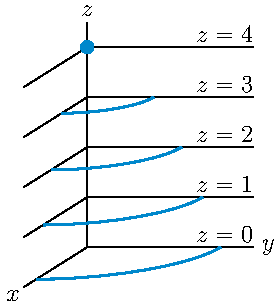
\includegraphics{fig/paraboloidGraphA.pdf}
\end{center}

\begin{center}
  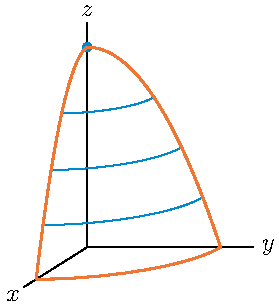
\includegraphics{fig/paraboloidGraphB.pdf}
\end{center}


\end{solution}


%%%%%%%%%%%%%%%%%%%%%%%%%%%%%%%%
\begin{question}
Sketch a few level curves for the function $f(x,y)$ whose graph $z=f(x,y)$
is sketched below.
\begin{center}
  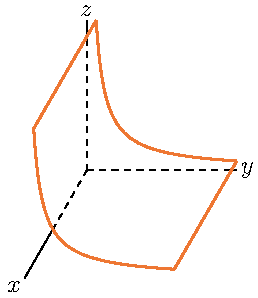
\includegraphics{fig/hyperCylinderGraph.pdf}
\end{center}
\end{question}

\begin{hint}
Draw in the plane $z=C$ for several values of $C$. 
\end{hint}


\begin{answer}
\begin{center}
  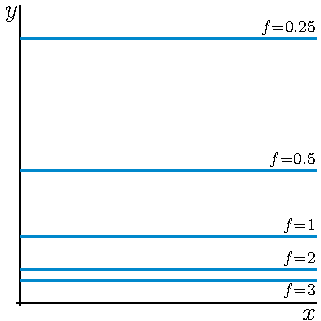
\includegraphics{fig/hyperCylinderLevel.pdf}
\end{center}
\end{answer}


\begin{solution}
We first add into the sketch of the graph the horizontal planes $z=C$,
for $C=3$, $2$, $1$, $0.5$, $0.25$. 
\begin{center}
  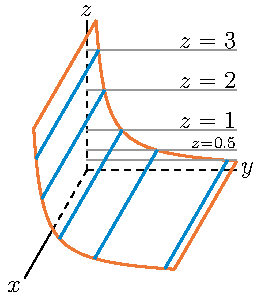
\includegraphics{fig/hyperCylinderGraphB.pdf}
\end{center}
To reduce clutter, for each $C$, we have drawn in only 
\begin{itemize}
\item 
the (gray) intersection of the horizontal plane $z=C$ with the $yz$--plane,
i.e. with the vertical plane $x=0$, and
\item
the (blue) intersection of the horizontal plane $z=C$ with the graph $z=f(x,y)$.
\end{itemize} 
We have also omitted the label for the plane $z=0.25$.

The intersection of the plane $z=C$ with the graph $z=f(x,y)$ is line
\begin{equation*}
\Set{(x,y,z)}{z=f(x,y),\ z=C} =  \Set{(x,y,z)}{f(x,y)=C,\ z=C}
\end{equation*}
Drawing this line (which is parallel to the $x$-axis) in the $xy$-plane,
rather than in the plane $z=C$, gives a level curve. Doing this for each of
$C=3$, $2$, $1$, $0.5$, $0.25$ gives five level curves. 
\begin{center}
  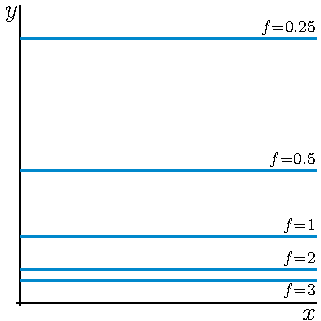
\includegraphics{fig/hyperCylinderLevel.pdf}
\end{center}

\end{solution}

%%%%%%%%%%%%%%%%%%%%%%%%%%%%
%\Instructions{Questions~\ref{prob_s1.0first} through \ref{prob_s1.0last} provide practice with.}
%%%%%%%%%%%%%%%%%%%%

%%%%%%%%%%%%%%%%%%
\subsection*{\Procedural}
%%%%%%%%%%%%%%%%%%

\begin{question}
Sketch some of the level curves of
\begin{enumerate}[(a)]
\item $f(x,y)=x^2+2y^2$
\item $f(x,y)=xy$
\item $f(x,y)=xe^{-y}$
\end{enumerate}

\end{question}

%\begin{hint}
%
%\end{hint}

\begin{answer}
(a)
\begin{center}
     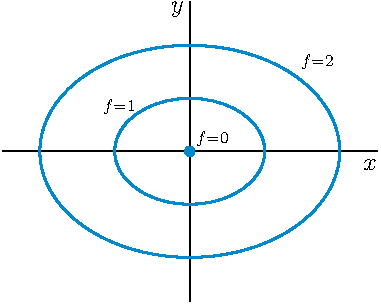
\includegraphics{fig/levelEllipse.pdf}
\end{center}

(b)
\begin{center}
     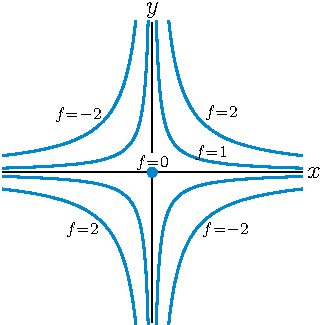
\includegraphics{fig/levelHyperbola.pdf}
\end{center}

(c)
\begin{center}
     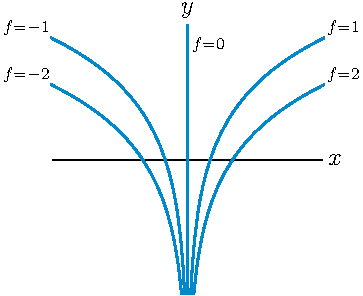
\includegraphics{fig/levelLog.pdf}
\end{center}

\end{answer}

\begin{solution} (a)
For each fixed $c>0$, the level curve $x^2+2y^2=c$ is the ellipse
centred on the origin with $x$ semi axis $\sqrt{c}$ and 
$y$ semi axis $\sqrt{c/2}$. If $c=0$,  the level curve $x^2+2y^2=c=0$
is the single point $(0,0)$.
\begin{center}
     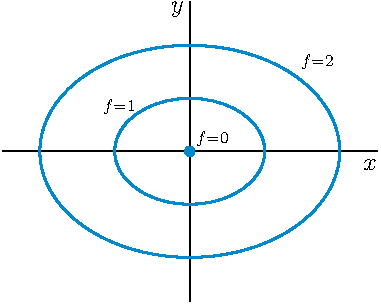
\includegraphics{fig/levelEllipse.pdf}
\end{center}

(b)
For each fixed $c\ne 0$, the level curve $xy=c$ is a hyperbola
centred on the origin with asymptotes the $x$- and $y$-axes. 
If $c>0$, any $x$ and $y$ obeying $xy=c>0$ are of the same sign.
So the hyperbola is contained in the first and third quadrants.
If $c<0$, any $x$ and $y$ obeying $xy=c>0$ are of opposite sign.
So the hyperbola is contained in the second and fourth quadrants.
If $c=0$,  the level curve $xy=c=0$
is the single point $(0,0)$.
\begin{center}
     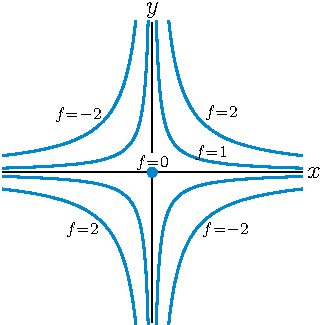
\includegraphics{fig/levelHyperbola.pdf}
\end{center}

(c)
For each fixed $c\ne 0$, the level curve $xe^{-y}=c$ is the logarithmic curve
$y=-\ln\frac{c}{x}$. Note that, for $c>0$, the curve
\begin{itemize}\itemsep1pt \parskip0pt \parsep0pt
\item is restricted to $x>0$, so that $\frac{c}{x}>0$ and $\ln \frac{c}{x}$
  is defined, and that
\item as $x\rightarrow 0^+$, $y$ goes to $-\infty$, while
\item as $x\rightarrow +\infty$, $y$ goes to $+\infty$, and
\item the curve crosses the $x$-axis (i.e. has $y=0$) when $x=c$.
\end{itemize}
and for $c<0$, the curve
\begin{itemize}\itemsep1pt \parskip0pt \parsep0pt
\item is restricted to $x<0$, so that $\frac{c}{x}>0$ and $\ln \frac{c}{x}$
  is defined, and that
\item as $x\rightarrow 0^-$, $y$ goes to $-\infty$, while
\item as $x\rightarrow -\infty$, $y$ goes to $+\infty$, and
\item the curve crosses the $x$-axis (i.e. has $y=0$) when $x=c$.
\end{itemize}
If $c=0$,  the level curve $xe^{-y}=c=0$
is the $y$-axis, $x=0$.
\begin{center}
     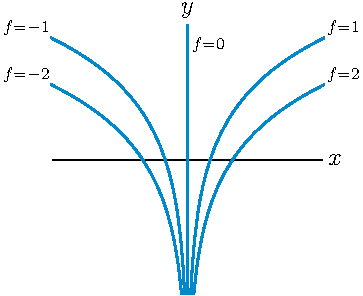
\includegraphics{fig/levelLog.pdf}
\end{center}



\end{solution}


%%%%%%%%%%%%%%%%%%%%%%%%%%%%%%%%

%%%%%%%%%%%%%%%%%%%%%%%%%%%%%%%%
\begin{question}[M200 2010D] %1a
Sketch the level curves of $f(x,y)=\frac{2y}{x^2+y^2}$.
\end{question}

%\begin{hint}
%
%\end{hint}

\begin{answer}
\begin{center}
     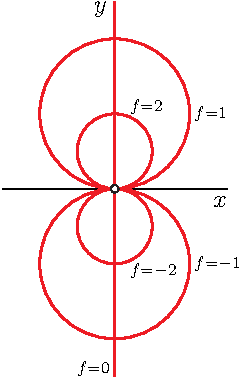
\includegraphics{fig/OE10D_1.pdf}
\end{center}
\end{answer}

\begin{solution}
 If $C=0$, the level curve $f=C=0$ is just the line $y=0$.
If $C\ne 0$ (of either sign), we may rewrite the equation, $f(x,y)=\frac{2y}{x^2+y^2}=C$,
of the level curve $f=C$ as 
\begin{equation*}
x^2-\frac{2}{C}y+y^2=0
\iff x^2+\left(y-\frac{1}{C}\right)^2 =\frac{1}{C^2} 
\end{equation*}
which is the equation of the circle of radius $\frac{1}{|C|}$ centred on
$\left(0\,,\,\frac{1}{C}\right)$.

\begin{center}
     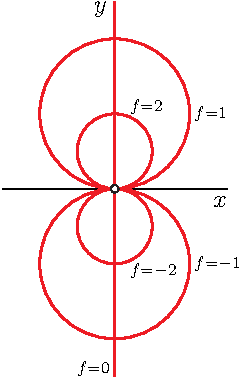
\includegraphics{fig/OE10D_1.pdf}
\end{center}

\emph{Remark.}\ \  
To be picky, the function $f(x,y)=\frac{2y}{x^2+y^2}$
is not defined at $(x,y)=(0,0)$. The question should have either specified
that the domain of $f$ excludes $(0,0)$ or have specified a value 
for $f(0,0)$. In fact, it is impossible to assign a value to $f(0,0)$
in such a way that $f(x,y)$ is continuous at $(0,0)$, because
$\lim_{x\rightarrow 0}f(x,0)=0$ while  $\lim_{y\rightarrow 0}f(0,|y|)=\infty$.
So it makes more sense to have the domain of $f$ being $\bbbr^2$  
with the point $(0,0)$ removed. That's why there is a little hole at the origin
in the above sketch.
\end{solution}


%%%%%%%%%%%%%%%%%%%%%%%%%%%%%%%%
\begin{question}[M200 2011D] %1a
Draw a ``contour map'' of $f(x, y) = e^{-x^2 +4y^2}$ , showing all types of level curves that occur.
\end{question}

%\begin{hint}
%
%\end{hint}

\begin{answer}
\begin{center}
     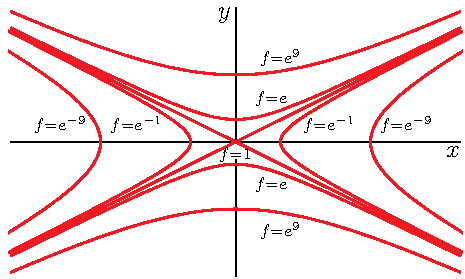
\includegraphics{fig/OE11D_1.pdf}
\end{center}
\end{answer}

\begin{solution}
 Observe that, for any constant $C$, the curve $-x^2+4y^2=C$
is the level curve $f=e^C$.
\begin{itemize}
\item
If $C=0$, then $-x^2+4y^2=C=0$ is the pair of lines $y=\pm\frac{x}{2}$.
\item
If $C>0$, then $-x^2+4y^2=C>0$ is the hyperbola $y=\pm\frac{1}{2}\sqrt{C+x^2}$. 
\item
If $C<0$, then $-x^2+4y^2=C<0$ is the hyperbola $x=\pm\sqrt{|C|+4y^2}$. 
\end{itemize}

\begin{center}
     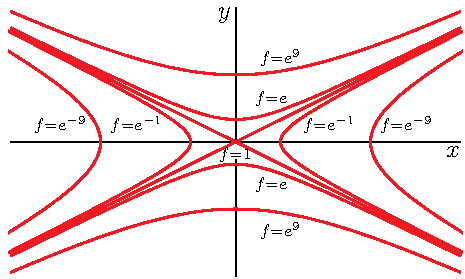
\includegraphics{fig/OE11D_1.pdf}
\end{center}

\end{solution}


%%%%%%%%%%%%%%%%%%%%%%%%%%%%%%%%
\begin{question}[M253 2011D] %1
A surface is given implicitly by
\begin{equation*}
x^2 + y^2 - z^2 + 2z = 0
\end{equation*}
\begin{enumerate}[(a)]
\item
Sketch several level curves $z = $constant.
\item
Draw a rough sketch of the surface. 
%\item
%Find the equation of the tangent plane to the surface at the point 
%$x = 2$, $y = 2$, $z = 4$.
\end{enumerate}
\end{question}

%\begin{hint}
%
%\end{hint}

\begin{answer}
(a)

\begin{center}
     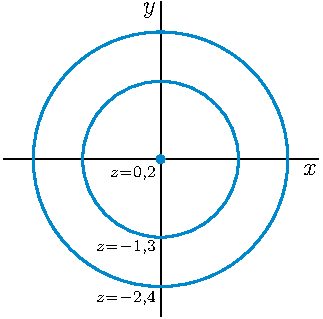
\includegraphics{fig/OE253_11D_1a.pdf}
\end{center}

(b)

\begin{center}
   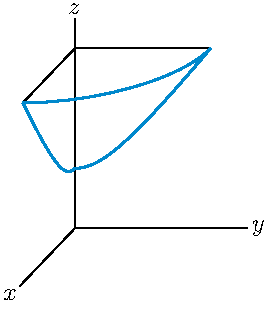
\includegraphics{fig/OE253_11D_1bl.pdf}\qquad\qquad
   \raisebox{0.1\height}{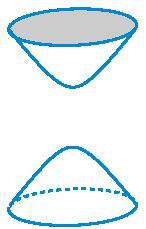
\includegraphics[scale=1.2]{fig/OE253_11D_1br.pdf}}
\end{center}
\end{answer}

\begin{solution} (a)
We can rewrite the equation as 
\begin{equation*}
x^2 + y^2 = (z-1)^2 - 1
\end{equation*}
The right hand side is negative for $|z-1|<1$, i.e. for $0<z<2$.
So no point on the surface has $0<z<2$. For any 
fixed $z$, outside that range, the curve $x^2 + y^2 = (z-1)^2 - 1$ 
is the circle of radius $\sqrt{(z-1)^2 - 1}$ centred on the $z$--axis.
That radius is $0$ when $z=0,2$ and increases as $z$ moves away from 
$z=0,2$. For very large $|z|$, the radius increases roughly linearly with
$|z|$. Here is a sketch of some level curves.

\begin{center}
     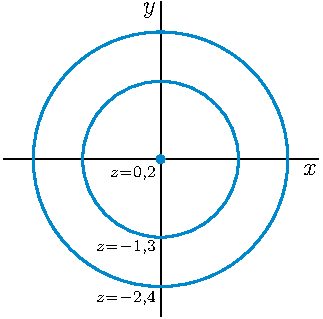
\includegraphics{fig/OE253_11D_1a.pdf}
\end{center}

(b)
The surface consists of two stacks of circles. 
One stack starts with radius $0$ at $z=2$. 
The radius increases as $z$ increases.
The other stack starts with radius $0$ at $z=0$. 
The radius increases as $z$ decreases.
This surface is a hyperboloid of two sheets. Here are two
sketchs. The sketch on the left is of the part of the surface in the
first octant. The sketch on the right of the full surface.

\begin{center}
   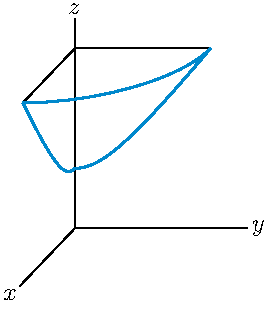
\includegraphics{fig/OE253_11D_1bl.pdf}\qquad\qquad
   \raisebox{0.1\height}{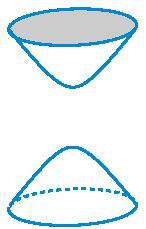
\includegraphics[scale=1.2]{fig/OE253_11D_1br.pdf}}
\end{center}

\end{solution}

%%%%%%%%%%%%%%%%%%%%%%%%%%%%%%%%
\begin{question}[M226 2009A] %1a
Sketch the hyperboloid $z^2=4x^2+y^2-1$.
\end{question}

%\begin{hint}
%
%\end{hint}

\begin{answer}
\begin{center}
   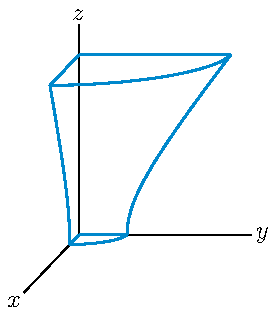
\includegraphics{fig/OE226_09A_l.pdf}\qquad\qquad
   \raisebox{0.1\height}{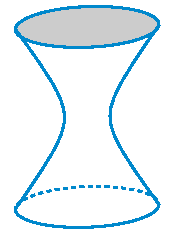
\includegraphics[scale=1.2]{fig/OE226_09A_r.pdf}}
\end{center}
\end{answer}

\begin{solution} 
For each fixed $z$, $4x^2+y^2=1+z^2$ is an ellipse. So the surface 
consists of a stack of ellipses one on top of the other. The semi axes are
$\frac{1}{2}\sqrt{1+z^2}$ and $\sqrt{1+z^2}$. These are smallest when $z=0$
(i.e. for the ellipse in the $xy$-plane) and increase as $|z|$ increases.
The intersection of the surface with the $xz$-plane (i.e. with the plane $y=0$) is the hyperbola $4x^2-z^2=1$ and the intersection with
the $yz$-pane (i.e. with the plane $x=0$) is the hyperbola $y^2-z^2=1$. 
Here are two sketches of the surface. The sketch on the left only shows 
the part of the surface in the first octant  (with axes).
\begin{center}
   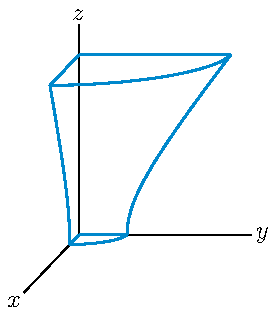
\includegraphics{fig/OE226_09A_l.pdf}\qquad\qquad
   \raisebox{0.1\height}{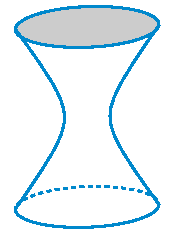
\includegraphics[scale=1.2]{fig/OE226_09A_r.pdf}}
\end{center}

\end{solution}

%%%%%%%%%%%%%%%%%%%%%%%%%%%%%%%%
\begin{question}
Describe the level surfaces of
\begin{enumerate}[(a)]
\item $f(x,y,z)=x^2+y^2+z^2$
\item $f(x,y,z)=x+2y+3z$
\item $f(x,y,z)=x^2+y^2$
\end{enumerate}
\end{question}

%\begin{hint}
%
%\end{hint}

\begin{answer}
(a)
 If $c>0$, $f(x,y,z)=c$
is the sphere of radius $\sqrt{c}$ centered at the origin. 
If $c=0$, $f(x,y,z)=c$ is just the origin. If $c<0$, no
$(x,y,z)$ satisfies $f(x,y,z)=c$.

(b) $f(x,y,z)=c$ is the plane normal to 
$(1,2,3)$ passing through $(c,0,0)$.

(c) If $c>0$, $f(x,y,z)=c$ is the cylinder 
parallel to the $z$-axis whose cross-section is a circle of 
radius $\sqrt{c}$ that is parallel to the $xy$-plane and is centered on the
$z$-axis. 
If $c=0$, $f(x,y,z)=c$ is the $z$-axis. If $c<0$, no
$(x,y,z)$ satisfies $f(x,y,z)=c$. 

\end{answer}

\begin{solution} (a)
 If $c>0$, $f(x,y,z)=c$, i.e. $x^2+y^2+z^2=c$, 
is the sphere of radius $\sqrt{c}$ centered at the origin. 
If $c=0$, $f(x,y,z)=c$ is just the origin. If $c<0$, no
$(x,y,z)$ satisfies $f(x,y,z)=c$. 

(b)  $f(x,y,z)=c$, i.e. $x+2y+3z=c$, is the plane normal to 
$(1,2,3)$ passing through $(c,0,0)$. 

(c) If $c>0$, $f(x,y,z)=c$, i.e. $x^2+y^2=c$, is the cylinder 
parallel to the $z$-axis whose cross-section is a circle of 
radius $\sqrt{c}$ that is parallel to the $xy$-plane and is centered on the
$z$-axis. 
If $c=0$, $f(x,y,z)=c$ is the $z$-axis. If $c<0$, no
$(x,y,z)$ satisfies $f(x,y,z)=c$. 

\end{solution}
%%%%%%%%%%%%%%%%%%%%%%%%%%%%%%%%

\begin{question}
Sketch the graphs of
\begin{enumerate}[(a)]
\item $f(x,y)=\sin x\qquad 0\le x\le 2\pi,\ 0\le y\le 1$
\item $f(x,y)=\sqrt{x^2+y^2}$
\item $f(x,y)=|x|+|y|$
\end{enumerate}

\end{question}

%\begin{hint}
%
%\end{hint}

\begin{answer}
(a) 
\begin{center}
     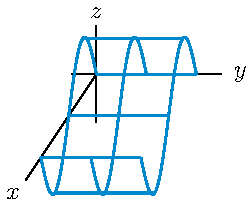
\includegraphics{fig/sinGraph.pdf}
\end{center}

(b) 
\begin{center}
     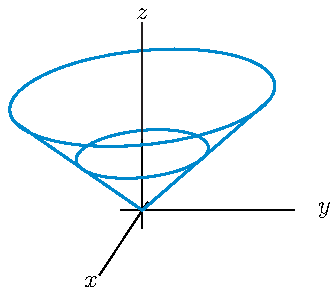
\includegraphics{fig/coneGraph.pdf}
\end{center}

(c)
\begin{center}
   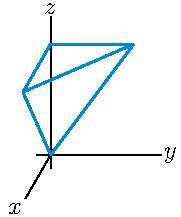
\includegraphics{fig/pmidGraph.pdf}\qquad\qquad
   \raisebox{0.1\height}{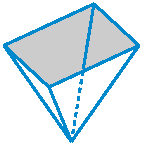
\includegraphics[scale=1.3]{fig/pmidGraphB.pdf}}
\end{center}
\end{answer}

\begin{solution} (a)
 The graph is $z=\sin x$ with $(x,y)$ running over
$0\le x\le 2\pi$,  $0\le y\le 1$. For each fixed $y_0$ between $0$ and $1$, 
the intersection of this graph with the vertical plane $y=y_0$ is the
same sin graph $z=\sin x$ with $x$ running from $0$ to $2\pi$. So the whole
graph is just a bunch of 2-d sin graphs stacked side-by-side. This gives
the graph on the left below.

\begin{center}
   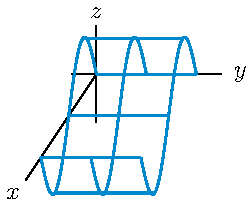
\includegraphics[scale=1.05]{fig/sinGraph.pdf}\qquad\qquad
   \raisebox{-0.1\height}{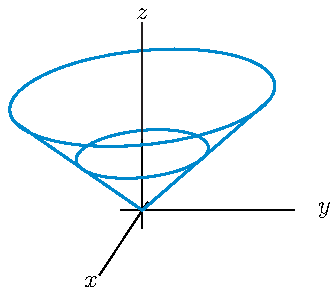
\includegraphics[scale=0.85]{fig/coneGraph.pdf}}
\end{center}

(b) 
The graph is $z=\sqrt{x^2+y^2}$. For each fixed $z_0\ge 0$, 
the intersection of this graph with the horizontal plane $z=z_0$ is the
circle $\sqrt{x^2+y^2}=z_0$. This circle is centred on the $z$-axis
and has radius $z_0$. So the graph is the upper half of a cone. It is the
sketch on the right above.

(c) 
The graph is $z=|x|+|y|$. For each fixed $z_0\ge 0$, 
the intersection of this graph with the horizontal plane $z=z_0$ is the
square $|x|+|y|=z_0$. The side of the square with $x,y\ge 0$ is the straight
line $x+y=z_0$. The side of the square with $x\ge 0$ and $y\le 0$ is 
the straight line $x-y=z_0$ and so on. The four corners of the square are
$(\pm z_0,0,z_0)$ and $(0, \pm z_0,z_0)$.  So the graph is a stack of squares.
It is an upside down four-sided pyramid. The part of the pyramid in the
first octant (that is, $x,y,z\ge 0$) is the sketch below.

\begin{center}
   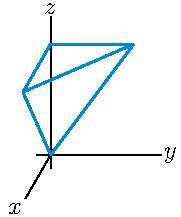
\includegraphics{fig/pmidGraph.pdf}\qquad\qquad
   \raisebox{0.1\height}{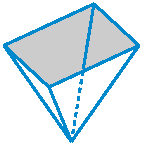
\includegraphics[scale=1.3]{fig/pmidGraphB.pdf}}
\end{center}

\end{solution}


%%%%%%%%%%%%%%%%%%%%%%%%%%%%%%%%


%%%%%%%%%%%%%%%%%%%%%%%%%%%%%%%%
\begin{question}
Sketch and describe the following surfaces.
\begin{enumerate}[(a)]
\item %a
$4x^2+y^2=16$

\item %b
$x+y+2z=4$  

\item %c
$\frac{y^2}{9}+\frac{z^2}{4}=1+\frac{x^2}{16}$ 

\item %d
$y^2=x^2+z^2$

\item %e
$\frac{x^2}{9}+\frac{y^2}{12}+\frac{z^2}{9}=1$

\item %f
$x^2+y^2+z^2+4x-by+9z-b=0$ where $b$ is a constant.

\item %g
 $\frac{x}{4}=\frac{y^2}{4}+\frac{z^2}{9}$ 

\item %h
$z=x^2$

%\item %i
%$z^2=y^2+4$

%\item %j
%$z=\frac{y^2}{4}-\frac{x^2}{9}$

\end{enumerate}

\end{question}

%\begin{hint}
%
%\end{hint}

\begin{answer}
(a) This is an elliptic cylinder parallel to the $z$-axis.
Here is a sketch of the part of the surface above the $xy$--plane.
\begin{center}
     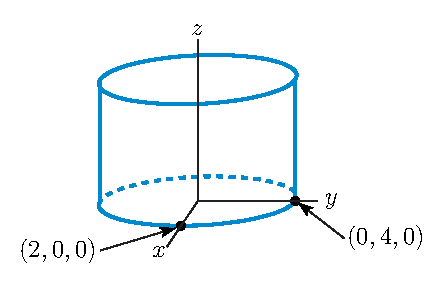
\includegraphics{fig/elliptical_cylinder}
\end{center}

(b)
This is a plane through $(4,0,0)$, $(0,4,0)$ and $(0,0,2)$.
Here is a sketch of the part of the plane in the first octant.
\begin{center}
     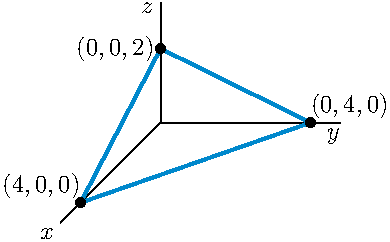
\includegraphics{fig/plane.pdf}
\end{center}

(c)
This is a hyperboloid of one sheet with axis the $x$-axis.
\begin{center}
     \includegraphics{fig/hyperboloidX_l.pdf}\qquad
     \includegraphics[scale=0.9]{fig/hyperboloidX_r.pdf}
\end{center}

(d)
This is a circular cone centred 
on the $y$-axis. 
\begin{center}
     \includegraphics{fig/coneYY_r.pdf}%\qquad
%     \includegraphics[scale=0.9]{fig/coneY_r.pdf}
\end{center}

(e)
This is an ellipsoid centered on the origin with semiaxes $3$, 
$\sqrt{12}=2\sqrt{3}$ and $3$ along the $x$, $y$ and $z$-axes, respectively.
\begin{center}
     \includegraphics{fig/ellipsoid_l.pdf}\qquad
     \includegraphics[scale=0.9]{fig/ellipsoid_r.pdf}
\end{center}

(f) 
This is a sphere of radius $r_b=\frac{1}{2}\sqrt{b^2+4b+97}$ centered on 
$\frac{1}{2}(-4,b,-9)$.
\begin{center}
     \includegraphics{fig/shiftSphere.pdf}
\end{center}

(g)
This is an elliptic paraboloid with axis the $x$-axis.
\begin{center}
     \includegraphics{fig/paraboloidX_l.pdf}\qquad
     \includegraphics[scale=0.8]{fig/paraboloidX_r.pdf}
\end{center}

(h)
This is an upward openning parabolic cylinder.
\begin{center}
     \includegraphics{fig/parabolicCylinder.pdf}
\end{center}

%(i)


\end{answer}

\begin{solution} 
(a) 
For each fixed $z_0$, the $z=z_0$ cross-section (parallel to the $xy$-plane) 
of this surface is an ellipse centered on the origin with
one semiaxis of length 2 along the $x$-axis and one semiaxis of length 
4 along the $y$-axis. So this is an elliptic cylinder parallel to the $z$-axis.
Here is a sketch of the part of the surface above the $xy$--plane.
\begin{center}
     \includegraphics{fig/elliptical_cylinder.pdf}
\end{center}

(b)
This is a plane through $(4,0,0)$, $(0,4,0)$ and $(0,0,2)$.
Here is a sketch of the part of the plane in the first octant.
\begin{center}
     \includegraphics{fig/plane.pdf}
\end{center}

(c)
For each fixed $x_0$, the $x=x_0$ 
cross-section parallel to the $yz$-plane is an ellipse with semiaxes 
$3\sqrt{1+\frac{x_0^2}{16}}$ parallel to the $y$-axis and
$2\sqrt{1+\frac{x_0^2}{16}}$ parallel to the $z$-axis. 
 As you move out along the $x$-axis, away from $x=0$, the ellipses grow
at a rate proportional to $\sqrt{1+\frac{x^2}{16}}$, which for large $x$
is approximately $\frac{|x|}{4}$.
This is called a hyperboloid of one sheet. Its 
\begin{center}
     \includegraphics{fig/hyperboloidX_l.pdf}\qquad
     \includegraphics[scale=0.9]{fig/hyperboloidX_r.pdf}
\end{center}

(d)
For each fixed $y_0$, the $y=x_0$ cross-section (parallel to the $xz$-plane) 
is a circle of radius $|y|$ centred on the $y$-axis. When $y_0=0$ the radius 
is $0$. As you move further from the $xz$-plane, in either direction, 
i.e. as $|y_0|$ increases, the radius grows linearly. The full surface 
consists of a bunch of these circles stacked sideways. This is a 
circular cone centred on the $y$-axis. 
\begin{center}
     \includegraphics{fig/coneYY_r.pdf}%\qquad
%     \includegraphics[scale=0.9]{fig/coneY_r.pdf}
\end{center}

(e)
This is an ellipsoid centered on the origin with semiaxes $3$, 
$\sqrt{12}=2\sqrt{3}$ and $3$ along the $x$, $y$ and $z$-axes, respectively.
\begin{center}
     \includegraphics{fig/ellipsoid_l.pdf}\qquad
     \includegraphics{fig/ellipsoid_r.pdf}
\end{center}

(f) 
Completing three squares, we have that
$x^2+y^2+z^2+4x-by+9z-b=0$ if and only if 
$(x+2)^2+\big(y-\frac{b}{2}\big)^2+\big(z+\frac{9}{2}\big)^2
=b+4+\frac{b^2}{4}+\frac{81}{4}$. 
This is a sphere of radius $r_b=\frac{1}{2}\sqrt{b^2+4b+97}$ centered on 
$\frac{1}{2}(-4,b,-9)$.
\begin{center}
     \includegraphics{fig/shiftSphere.pdf}
\end{center}


(g)
There are no points on the surface with $x<0$.
For each fixed $x_0>0$ the cross-section $x=x_0$ parallel to the
$yz$-plane is an ellipse centred on the $x$--axis with semiaxes $\sqrt{x_0}$ 
in the $y$-axis direction and $\frac{3}{2}\sqrt{x_0}$ in the $z$--axis
direction.  As you increase $x_0$, i.e. move out along the $x$-axis, 
the ellipses grow at a rate proportional to $\sqrt{x_0}$. This is 
an elliptic paraboloid  with axis the $x$-axis.
\begin{center}
     \includegraphics{fig/paraboloidX_l.pdf}\qquad
     \includegraphics[scale=0.8]{fig/paraboloidX_r.pdf}
\end{center}


(h)
This is called a parabolic cylinder. For any fixed $y_0$, the  
$y=y_0$ cross-section (parallel to the $xz$-plane) is the upward
opening parabola $z=x^2$ which has vertex on the $y$-axis.
\begin{center}
     \includegraphics{fig/parabolicCylinder.pdf}
\end{center}

%(i)
%For each fixed $x_0$, the $x=x_0$ cross-section (parallel to the $yz$--plane) 
%is the hyperbola $z^2=y^2+4$. It is centered on the origin and has
%asymptotes $z=\pm y$. No points have $|z|< 2$.
%This is a hyperbolic cylinder parallel to the $x$-axis.
%\begin{center}
%     \includegraphics{fig/hyperbolicCylinder.pdf}
%\end{center}

%(j)
%This is called a hyperbolic paraboloid. Each cross-section
%parallel to the $xz$-plane is a parabola opening downwards, with vertex
%at $(0,y,\frac{y^2}{4})$. Each cross-section
%parallel to the $yz$-plane is a parabola opening upwards, with vertex
%at $(x,0,-\frac{x^2}{9})$. Each cross--section
%parallel to the $xy$-plane is a hyperbola with asymptotes $y=\pm\frac{2}{3}x$.
%\begin{center}
%     \includegraphics{fig/hyperbolic_paraboloid.pdf}
%\end{center}




\end{solution}






%%%%%%%%%%%%%%%%%%
\subsection*{\Application}
%%%%%%%%%%%%%%%%%%
%%%%%%%%%%%%%%%%%%%
\begin{question}
The surface below has circular level curves, centred along the $z$-axis. The lines given are the intersection of the surface with the right half of the $yz$-plane. Give an equation for the surface.
\begin{center}
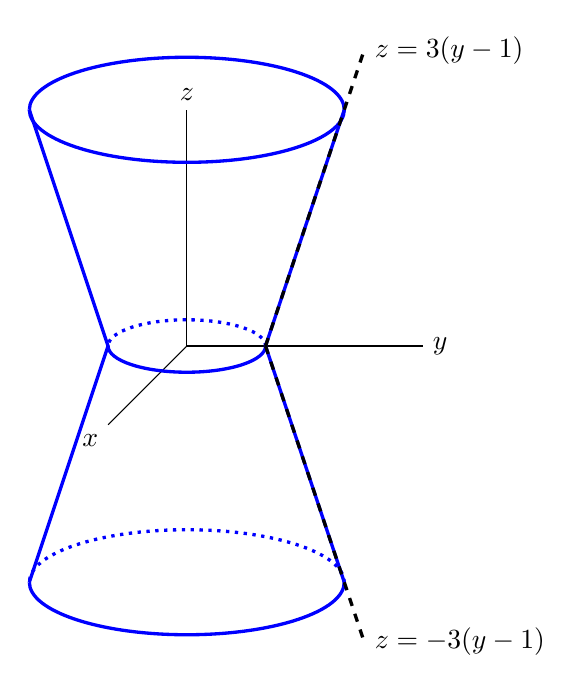
\begin{tikzpicture}
\draw (0,0)--(0,3)node[above]{$z$};
\draw (0,0)--(3,0) node[right]{$y$};
\draw (0,0)--(-1,-1) node[below left]{$x$};


\draw[very thick,blue] (1,0) arc (360:180:1cm and .333 cm);
\draw[dotted, very thick, blue] (1,0) arc (0:180:1cm and .333 cm);

\draw[very thick,blue] (2,3) arc (360:180:2cm and .667 cm);
\draw[very thick,blue] (2,3) arc (0:180:2cm and .667 cm);

\draw[very thick,blue] (2,-3,0) arc (360:180:2cm and .667 cm);
\draw[dotted, very thick, blue] (2,-3) arc (0:180:2cm and .667 cm);

\draw[very thick, blue] (2,-3)--(1,0)--(2,3) (-2,-3)--(-1,0)--(-2,3);

\draw[very thick, dashed] (1,0)--(2.25,3.75)node[right]{$z=3(y-1)$};
\draw[very thick, dashed] (1,0)--(2.25,-3.75)node[right]{$z=-3(y-1)$};

\end{tikzpicture}
\end{center}
\end{question}
\begin{hint}
Since the level curves are circles centred at the origin (in the $xy$-plane), the equation will have the form $x^2+y^2=g(z)$, where $g(z)$ is a function depending only on $z$.
\end{hint}
\begin{answer}
$\displaystyle x^2+y^2=\left( \frac{|z|}{3}+1\right)^2$
\end{answer}
\begin{solution}
Since the level curves are circles centred at the origin (in the $xy$-plane), when $z$ is a constant, the equation will have the form $x^2+y^2=c$ for some constant. That is, our equation looks like
\[x^2+y^2=g(z),\] where $g(z)$ is a function depending only on $z$.


Because our cross-sections are so nicely symmetric, we know the intersection of the figure with the left side of the $yz$-plane as well: $z=3(-y-1)=-3(y+1)$ 
(when $z\ge0$) and $z=-3(-y-1)=3(y+1)$ (when $z<0$). Below is the intersection of our surface with the $yz$ plane.

\begin{center}
\begin{tikzpicture}
\draw (0,-3)--(0,3)node[above]{$z$};
\draw (-3,0)--(3,0) node[right]{$y$};
%\draw (0,0)--(-1,-1) node[below left]{$x$};

\draw[very thick, dashed] (1,0)--(2.25,3.75)node[right]{$z=3(y-1)$};
\draw[very thick, dashed] (1,0)--(2.25,-3.75)node[right]{$z=-3(y-1)$};

\draw[very thick, dashed] (-1,0)--(-2.25,3.75)node[left]{$z=-3(y+1)$};
\draw[very thick, dashed] (-1,0)--(-2.25,-3.75)node[left]{$z=3(y+1)$};

\end{tikzpicture}
\end{center}

Setting $x=0$, our equation becomes $y^2=g(z)$. Looking at the right side of the $yz$ plane, this should lead to:
$\left.\begin{cases}
z=3(y-1) &\mbox{if } z\geq 0,\ y\ge 1\\
z=-3(y-1) &\mbox{if } z< 0,\ y\ge 1
\end{cases}\right\} $. That is:

\begin{align*}
|z|&=3(y-1)\\
\frac{|z|}{3}+1&=y\\
\left(\frac{|z|}{3}+1\right)^2&=y^2 &(*)
\end{align*}

A quick check: when we squared both sides of the equation in $(*)$, we added another solution, $\frac{|z|}{3}+1=-y$. Let's make sure we haven't diverged from our diagram.

\begin{align*}
&&& \left(\frac{|z|}{3}+1\right)^2=y^2\\
&\Leftrightarrow&& \underbrace{\frac{|z|}{3}+1}_{\text{positive}}=\pm y\\
&\Leftrightarrow&& \begin{cases}
 \frac{|z|}{3}+1 =y & y>0\\[0.05in]
  \frac{|z|}{3}+1 =-y & y<0
 \end{cases}\displaybreak[0]\\[0.1in]
& \Leftrightarrow&& \begin{cases}
 \frac{|z|}{3}+1 =y & y\ge1\\[0.05in]
  \frac{|z|}{3}+1 =-y & y\le-1
 \end{cases}\displaybreak[0]\\[0.1in]
&\Leftrightarrow&&  \begin{cases}
|z| =3(y-1) & y\ge1\\[0.05in]
|z|=-3(y+1) & y\le-1
 \end{cases}\displaybreak[0]\\[0.1in]
&\Leftrightarrow&&  \begin{cases}
z =\pm \underbrace{3(y-1)}_{\text{positive}} & y\ge1\\
z=\pm \underbrace{3(y+1)}_{\text{negative}} & y\le-1
 \end{cases}\displaybreak[0]\\[0.1in]
&\Leftrightarrow&&  \begin{cases}
z =3(y-1) & y\ge1,\ z\ge0\\
z =-3(y-1) & y\ge1,\ z\le0\\
z=-3(y+1) & y\le-1,\ z \ge 0\\
z=3(y+1) & y\le-1,\ z\le 0
 \end{cases}
\end{align*}

This matches our diagram eactly. So, all together, the equation of the surface is
\[x^2+y^2=\left( \frac{|z|}{3}+1\right)^2\]
\end{solution}
%%%%%%%%%%%%%%%%%%%
